\chapter{Step 2: Policy Alternative Determination}\label{dev-step2}

\begin{abstract}
    The second step in an RDM-based analysis is the policy alternative determination process, also referred to as the search phase. This research divides step 2 into three distinct parts. \cref{step2-moea} will establish the search algorithm that is used to find policy alternatives. Next, the different mechanisms for comparing potential alternatives is discussed in \cref{step2-scenarios}. Because this research includes seed analysis to manage the impact of randomness on the MOEA search, the final stage, \cref{step2-pareto} describes the process in which alternatives that are identified in each search repetition are put through a final selection process using an $\epsilon$-based Pareto sorting algorithm. 
\end{abstract}

\medskip

\begin{figure}[h]
    \centering
    \captionsetup{justification=centering}
    
    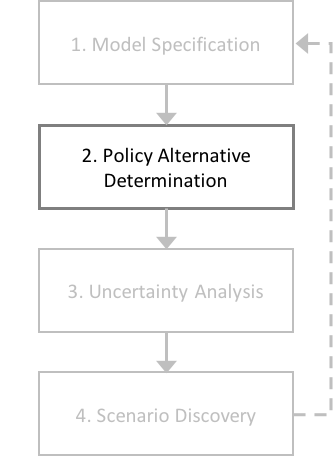
\includegraphics{structure-step2}
    \caption{RDM Structure - Step 2}
    \label{fig:structure-step2}
\end{figure}

\newpage

\section{Multi-Objective Evolutionary Algorithms (MOEAs)} \label{step2-moea}
Wicked problems characterized by tipping point behavior will generally involve multiple conflicting objectives due to their deeply uncertain nature. Because of this, there is no single optimal solution to these problems; instead, analysts must look for a set of potential alternatives, where each solution in the set is not dominated by any other solution in the set. This is known as Pareto optimality. To find the Pareto optimal set of solutions, analysis requires a search algorithm that is capable of handling conflicting objectives. The most common solution is what's known as a multi-objective evolutionary algorithm \citep{Maier2014, Reed2013}. A multi-objective evolutionary algorithm (MOEA) is one that takes a generic approach to optimization, where a population of potentially optimal items is generated through an iterative process of the following steps: 

\indent\textbf{Begin}: 
\begin{enumerate}[start=0]
    \item A set of options is randomly determined, the fitness of of which is determined based on the case-specific definition provided.
\end{enumerate}

\indent\textbf{Iterative Steps}: 
\begin{enumerate}[start=1]
    \item The most fit options are used to generate new options for consideration - the next generation of alternatives. 
    \item Fitness of those new options is determined using the same definition as in 0. 
    \item The options with the lowest fitness in the existing set are replaced with items of higher fitness in the newly discovered set. 
\end{enumerate}

Many MOEAs have been developed over the years, each of which aims to discover potential solutions to multi-objective problems. One of the earliest examples, NSGAII, is a generational algorithm that was developed by \citet{Deb2002}. A general MOEA replaces the entire population of currently tracked solutions after every search iteration \citep{Reed2013}. NSGAII uses a constant population size for each generation, and was one of the earliest to use Pareto dominance to search for and rank alternative solutions to a provided problem. 

After each search iteration, NSGAII uses a Pareto sorting algorithm to find the new population of non-dominated solutions when combining the existing set of solutions and the newly found population of potential alternatives. This results in a new set of non-dominated alternatives that is used in the next iteration \citep{Reed2013}. The goal of this search process is to find a set of non-dominated solutions that make up the Pareto optimal front, which would precisely describe the complex trade-offs between conflicting objectives. Due to the presence of uncertain behavior and conflicting objectives, however, it is impossible to reach the optimal front precisely. Therefore, the search process determines what is called an approximation of the Pareto front.  

To facilitate the search process, NSGAII makes use of a single operator that is responsible for maintaining diversity of solutions \citep{Reed2013, Ward2015}. The NSGAII algorithm has had solid performance in many optimization problems and is therefore still commonly used today \citep{Zheng2016}. 

The NSGAII algorithm was extended to create $\epsilon$-NSGAII by incorporating epsilon dominance in the sorting process and by using adaptive population sizing across the different generations. Together, these two characteristics have shown to reduce the need for extensive calibration of input parameters and to include more efficient search process \citep{Ward2015}. Epsilon dominance enables the decision maker to specify her desired level of precision for a policy to be considered dominant for each outcome of interest. With this property, solutions are only considered dominant if they fall outside the space defined by the epsilon value of an outcome of interest \citep{Horoba2008}. This allows for the elimination of alternatives that are considered similar and encourages diversity in the final set of recommended options \citep{Reed2013}. An epsilon value of 0 means that the Pareto sorting algorithm will behave similarly to one without any epsilon dominance considerations, as is found in traditional NSGAII. 

Along with epsilon dominance, adaptive population sizing allows for a more efficient search to be completed. The number of alternatives being tested can begin with a smaller population size to reduce computational cost. Once a more stable set of alternatives has been generated, the population size can be increased to put more pressure on the fitness and selection process, which ensures that the most fit solutions are being found in each generation \citep{Ward2015}. Other traditionally structured MOEA algorithms include SPEA2, $\epsilon$-MOEA, OMOPSO, MOEA/D, and GDE3 \citep{Reed2013, Ward2015, Zheng2016}. Each of these algorithms use a constant operator and some form of Pareto dominance to find solutions and maintain diversity.

An alternative to these traditional algorithms is a hybrid-MOEA known as Borg, which is built on the $\epsilon$-MOEA algorithm, a steady-state MOEA. Unlike a generational algorithm, a steady-state MOEA attempts to replace one solution in the existing set of alternative solutions after each search iteration, creating a highly efficient search process \citep{Ward2015}. 

Borg pairs the ideas of adaptive population sizing and epsilon dominance used in $\epsilon$-MOEA with a new auto-adaptive operator selection process and randomized algorithm restarts when search progress stalls to efficiently find well-performing solution alternatives \citep{HadkaReed2013}. By using auto-adaptive operator selection, as opposed to a single operator used as is used in earlier search algorithms, Borg is able to use operators based on their ability to select the strongest candidate solutions, leading to a more efficient and effective search process. The randomized restart function enables Borg, upon detecting that the search process has stalled, to inject new and diverse alternatives into the search process, ensuring the best chance for a diverse set of alternatives that more closely approximates the optimal Pareto front once the algorithm completes its run \citep{Reed2013}. 

Several studies have been completed that compare the success or failure of various MOEAs for a variety of policy problems. These studies have generally concluded that the auto-adaptive operator selection and adaptive population sizing together allow Borg to identify a more robust and diverse set of alternatives than other methods \citep{Reed2013, Ward2015, Zheng2016}. Algorithms apart from Borg that achieved at least some success are $\epsilon$-MOEA, NSGAII, and $\epsilon$-NSGAII, but none of these algorithms have provided results at the level of Borg. 

    \subsection{Auto-adaptive $\epsilon$-NSGAII} \label{hybridnsgaii}
    While Borg has been discovered to be quite successful at find a strong approximation of a problem's Pareto optimal front, it does so by leveraging a steady-state genetic algorithm. In this type of algorithm, only one new alternative is generated and folded into the existing non-dominated set at a time. This requires strategies to both select the desired parents from the existing set of alternatives and to prescriptively replace solutions in the existing set, both actions of which can significantly impact the outcome of the search process \citep{Vavak1996}, leading to the potential for additional uncertainty in analysis of a problem already fraught with uncertainty. Slow replacement of the non-dominated set can also contribute to slower convergence to the Pareto-optimal front \citep{Vavak1996}. 
    
    In contrast, a generational algorithm uses a much larger portion of the existing set of non-dominated solutions in each iteration of the search process to generate a new set of alternatives. These two sets are then compared to build an entirely new set of alternative solutions at the end of each iteration. This can lead to a faster convergence toward the Pareto optimal front \citep{Vavak1996}. 
    
    This research proposes an advancement of the traditional $\epsilon$-NSGAII algorithm that combines the strongest attributes of Borg: auto-adaptive operator selection and adaptive population sizing, with the best attributes of $\epsilon$-NSGAII: epsilon-dominance and a generational algorithm that has fast convergence to the Pareto optimal front. Instead of using a single operator as in the traditional $\epsilon$-NSGAII algorithm, auto-adaptive $\epsilon$-NSGAII uses a selection process similar to Borg to select an operator from the same group of operators that Borg considers. Each operator is assigned a probability of selection based on the number of solutions that an operator has produced that end up in the non-dominated set of alternatives after each search iteration. Operator elements and their parameter settings are indicated in \cref{table:nsgaii-hybrid}, and the complete operator definitions are listed below. 

    \begin{itemize}
        \item Simulated Binary Crossover (SBX) variator + Polynomial Mutation (PM) mutator
        \item Parent-centric Crossover (PCX) variator + PM mutator
        \item Differential Evolution (DE) variator + PM mutator
        \item Unimodal Normal Distribution Crossover (UNDX) variator + PM mutator
        \item Simplex Crossover (SPX) variator + PM mutator
        \item Uniform mutation (UM) mutator
    \end{itemize}

    \begin{table}[ht]
        \centering
        \captionsetup{width=0.57\textwidth}
        \caption[Auto-adaptive $\epsilon$-NSGAII configuration]{A sumary of the configuration details for the variant and mutator elements of the operators used in the proposed auto-adaptive NSGAII algorithm \citep{HadkaReed2013}}
        \label{table:nsgaii-hybrid}
        
        \setlength\arrayrulewidth{1pt}\arrayrulecolor{white}
        \rowcolors{2}{odd-row-blue}{even-row-blue}
        \begin{tabularx}{0.55\textwidth}{|l|X|r|}
            \rowcolor{tudelft-dark-blue!80}
            \color{white}\bfseries Name      &   \color{white}\bfseries Property Name   &   
            \multicolumn{1}{|l|}{\color{white}\bfseries Value} \\ \hline
            
                                   & probability            & $1.0 / L$        \\ \cline{2-3} 
            \multirow{-2}{*}{PM}   & distribution index     & $20$             \\ \hline
                                   & probability            & $1.0$            \\ \cline{2-3} 
            \multirow{-2}{*}{SBX}  & distribution index     & $15$             \\ \hline
                                   & nparents               & $3$              \\ \cline{2-3} 
                                   & noffspring             & $2$              \\ \cline{2-3} 
                                   & eta                    & $0.1$            \\ \cline{2-3} 
            \multirow{-4}{*}{PCX}  & Zeta                   & $0.1$            \\ \hline
                                   & crossover rate         & $0.1$            \\ \cline{2-3} 
            \multirow{-2}{*}{DE}   & step size              & $0.6$            \\ \hline
                                   & nparents               & $3$              \\ \cline{2-3} 
                                   & noffspring             & $2$              \\ \cline{2-3} 
                                   & zeta                   & $0.5$            \\ \cline{2-3} 
            \multirow{-4}{*}{UNDX} & eta                    & $0.35/\sqrt{L}$   \\ \hline
                                   & nparents               & $L+1$            \\ \cline{2-3} 
                                   & noffspring             & $L+1$            \\ \cline{2-3} 
            \multirow{-3}{*}{SPX}  & expansion              & $\sqrt{(L+1)+1}$  \\ \hline
            UM                     & probability            & $1.0/L$          \\
        \end{tabularx}
    \end{table}

    Alternative solutions are identified in the search process using tournament selection logic similar to what is found with the original $\epsilon$-NSGAII algorithm. As auto-adaptive $\epsilon$-NSGAII includes adaptive population sizing, the number of alternatives involved in each iteration of the tournament selection will change to match the size of the previously identified set of non-dominated alternative solutions. The initial population is determined using a Latin Hypercube sampling to build a set of alternatives based on the desired initial population size. A Latin Hypercube sampling ensures that each member of the decision lever set is represented evenly across the initial population \citep{Mckay1979}. In the case of this study, the initial population size will be 100. 
    
    The complexity of deeply uncertain problems and the large number of function executions needed mean that significant computing power is required for the MOEA to efficiently find as close an approximation to the Pareto front as possible. This can be accomplished through parallel computing. Borg, and other steady-state MOEAs can be parallelized through what is known as a master-slave architecture, in which a "master" process generates sub-problems that can run independently in their own processes. The results of these sub-problems are then returned to the master \citep{Zavoianu2013}. Such a scheme allows for a Borg-based search to make efficient use of CPU resources, as each sub-process is able to independently evaluate a single solution for potential replacement. However, there are limitations to the number of sub-processes that can be started at once to avoid  evaluating too many solution alternatives at the same time \citep{Hadka2013}. Furthermore, there is significant work required to develop a high-quality master-slave system to support parallelization of steady-state MOEAs \citep{Hadka2015Scale}. Parallelizing a generational algorithm like the proposed auto-adaptive NSGAII MOEA is much more straight forward, as each population member is independent from the others, with each iteration of the search process producing a new and independent population of alternatives with which to compare. Therefore, it is much simpler to take advantage of the computing power brought by parallelization for the proposed auto-adaptive $\epsilon$-NSGAII algorithm. A potential bottleneck does exist with a generational MOEA when the new population must be compared to the same existing set of non-dominated alternatives. Computational cost can be reduced here by using as efficient a Pareto sorting algorithm as possible. 
    
    The auto-adaptive $\epsilon$-NSGAII algorithm used for this study is implemented using the existing functions from the Python-based Platypus optimization package, which is a Python clone of the Java-based MOEAFramework. Platypus contains existing implementations of an epsilon-based search process, multi-operator management, tournament selection to determine potential solutions, and a Pareto-based sort to build the set of non-dominated solution alternatives. These pieces are combined to create the new auto-adaptive $\epsilon$-NSGAII algorithm. At the time of this thesis, Borg requires a paid license or special dispensation to use. Because the algorithm leverages existing open-source code, it is freely available for anyone to leverage in their own analysis. Details about where to find the implementation can be found in \cref{appendix-code}.

    \subsection{MOEA configuration}
    The auto-adaptive $\epsilon$-NSGAII algorithm is used for all three methods of robust decision support. Apart from the evaluation mechanism, which is discussed in \cref{step2-scenarios}, algorithm configuration is consistent across all methods under consideration to ensure a fair comparison by limiting the differences between methods as much as possible. Configuration is based on the parameters in \cref{table:moeaadditional}. This table also includes epsilon value settings, which were determined through referencing past research that has used the lake problem \citep{Quinn2017,Ward2015}, and by balancing the computational cost of having smaller epsilon values with the added benefit that smaller values may yield a closer approximation of the Pareto front. A study of the impact of different epsilon values on the search results for MORDM can be found in \cref{appendix-epsilon}. Traditionally, however, epsilon values are determined with input from the decision maker, who are able to indicate there preference for fine-grained control and computational efficiency. 

    \begin{table}[ht]
    \caption{Additional Configuration for the MOEA-based search}
    \label{table:moeaadditional}
    
    \setlength\arrayrulewidth{1pt}\arrayrulecolor{white}
    \rowcolors{2}{odd-row-blue}{even-row-blue}
    \begin{tabularx}{\textwidth}{|l|X|l|}
        \rowcolor{tudelft-dark-blue!80}
        \color{white}\bfseries Name          &
        \color{white}\bfseries Description   &
        \color{white}\bfseries Setting
        \\  \hline
        
        Population     & Starting number of policy alternatives that are tested each generation   & 100 \\ \hline
        
        \multicolumn{3}{|c|}{\cellcolor{tudelft-dark-blue!50}\color{white}Number Function Executions} \\ \hline
                                             & MORDM, multi-Scenario MORDM       & 500,000  \\ \cline{2-3} 
        \multirow{-2}{*}{Intertemporal}      & MORO                              & 300,000  \\ \hline
        Planned Adaptive DPS                 & All Methods                       & 100,000  \\ \hline
        DPS                                  & All Methods                       & 100,000  \\ \hline
        
        \multicolumn{3}{|c|}{\cellcolor{tudelft-dark-blue!50}{\color{white} Convergences}}  \\ \hline
        Epsilon Progress        & \multicolumn{2}{l|}{An indication of the search progress}           \\ \hline
        Operator Usage          & \multicolumn{2}{l|}{Usage of each operator as the search continues} \\ \hline
        \cellcolor{even-row-blue}    & MORDM                      & {[}2.5, 2, 1, 1{]}          \\ \cline{2-3} 
        \cellcolor{even-row-blue}    & Multi-Scenario MORDM       & {[}10, 2, 1, 1{]}           \\ \cline{2-3} 
        \multirow{-3}{*}{\cellcolor{even-row-blue}{ Hypervolume Limits}}  & MORO   & {[}1, 1, 1, 1{]} \\ \hline
        
        \multicolumn{3}{|c|}{\cellcolor{tudelft-dark-blue!50}{\color{white} Epsilon Settings}}  \\ \hline
        \multicolumn{2}{|l|}{Pollution Level}           & 0.1                                   \\ \hline
        \multicolumn{2}{|l|}{Utility}                   & 0.1                                   \\ \hline
        \multicolumn{2}{|l|}{Inertia}                   & 0.01                                  \\ \hline
        \multicolumn{2}{|l|}{Reliability}               & 0.01                                  \\
    \end{tabularx}
    \end{table}

    There are two small differences in configuration that are a part of \cref{table:moeaadditional}. Each of the problem iterations has its own setting for the number of function executions required for a single search to be completed. This number was established through testing of different values and was made large enough to ensure consistent convergence to a steady set of solution alternatives across independent search runs. The intertemporal variation of the lake problem requires a significantly larger number of function executions due to the much larger number of decision levers present in that variation (see \cref{step1-L} for details). The number of function executions configured for the intertemporal variation and MORO method pairing is lower than for the other two methods due to computational constraints, but consistent convergence was still achieved. 
    
    The second difference is in the hypervolume limits established for the convergence metrics. These values were established after testing of each robust decision support method and represent the approximate maximum values for each outcome of interest in the following order [pollution level, utility, inertia, reliability]. The hypervolume convergence metric does not affect the search process itself, but provides a mechanism for tracking stabilization of the search process. Hypervolume will be discussed further in \cref{results-convergence}. 

\section{Mechanism for Evaluation} \label{step2-scenarios}
The most critical element when configuring the search phase is the manner in which policies will be compared. Each of the RDM-based methods considered here have a different mechanism with which to accomplish this. MORDM and multi-scenario MORDM both use one reference scenario (at a time, in the case of multi-scenario MORDM) to test a policy against. The resulting values of the outcomes of interest are then used in the non-dominated selection process of the MOEA. In contrast, MORO test a policy against a set of scenarios and determines fitness by evaluating the robustness of the policy using the resulting sets of outcomes. These processes will be explained in more detail next. 

    \subsection{MORDM} \label{step2-mordm}
    MORDM is the earliest extension of the RDM method that introduced a formal mechanism to handle multiple conflicting objectives, through a multi-objective evolutionary algorithm-based search. Alternative policies that have been identified are compared in MORDM based on their performance in a single static reference scenario \citep{Kasprzyk2013}. That scenario is generally determined through conversation with decision makers, but in this case is based on the configuration used by \citep{Quinn2017}. Specific base values are found in \cref{table:uncertainties}. Policies are placed in the set of non-dominated options if they lead to stronger performance in that base scenario. This mechanism of evaluation, therefore, does not directly or indirectly incorporate robustness in the evaluation of alternatives. 

    \subsection{Multi-Scenario MORDM}
    As indicated in \cref{review-multi}, the fundamental difference between the MORDM and multi-Scenario MORDM methods is the repetition of the search process (as well as uncertainty analysis and scenario discovery) using more than one reference scenario. \cref{review-multi} discussed many potential ways to select the set of reference scenarios. This research uses a combination of two key techniques to select four scenarios that, when used in combination with the base reference scenario identified in \cref{step2-mordm}. The first is to leverage the uncertainty space that is revealed to cause vulnerabilities in policies found through the scenario discovery process in traditional MORDM, similar to the process discussed by \citet{Watson2017}. The second technique is to select a set of four maximally diverse scenarios from within a larger set of scenarios that fall within the identified vulnerable uncertainty space, as \citet{Eker2018} discussed. Specifically, this process involves steps listed below.
    
    \begin{enumerate}[leftmargin=*]
        \item Perform traditional MORDM-based analysis with a single reference scenario through the scenario discovery process. 
        \item Build a library of experiments that include uncertainty settings and how each set of uncertainty values respond under a group of different policies. This study examines how 500 sets of uncertainty values respond to a set of 10 different policies. These policies were determined by sampling across the lever space using a Latin Hypercube technique. The library of experiments will be used to select the four additional reference scenarios used in analysis. 
        \item Use the results of the scenario discovery process to select a subset of experiments with parameters that fall in the vulnerable ranges identified in scenario discovery. This subset of experiments will be used in the selection of four maximally diverse scenarios. 
        \item Given the subset of policy options, perform an exhaustive search of all possible combinations of four different policies to discover the maximally diverse set, based on the outcomes of interest. Diversity is determined in the same way as \citep{Eker2018}, who use euclidean distance between normalized values of the outcome indicators. Specifically, distance of a set of four policies is defined as in \cref{eq:step2-maxdistance} \citep{Carlsen2016}. The final set of policies selected is the one who has the largest calculated distance.
    \end{enumerate}
    
    \begin{equation}\label{eq:step2-maxdistance}
    distance = 1/2 * \underset{\forall j,k \in set}{min}{d_{k,j}} + 
               1/2 * \underset{\forall j,k \in set}{mean} {d_{k,j}}
    \end{equation}
    \begin{equation}\label{eq:step2-distancedef}
     d_{k,j} = \sqrt{\sum_{i} (\bar{o_{i,j}} - \bar{o_{i,k}})^{2}}
    \end{equation}

    The identified reference scenarios for each model variation are visualized in \cref{fig:selected-scenarios} and described in \cref{table:refscenario-inter,table:refscenario-adapt,table:refscenario-dps}. For all model variations, values are selected from the bottom half of the ranges for uncertainty parameters that relate to the removal of pollution from the lake, b and q, indicating that the policies discovered by the MORDM analysis tend to fail when the lake is not as successful at removing pollution on it's own. Values are selected from a a wide range for the other three uncertainty parameters. Also of note, the planned adaptive DPS variation revealed fewer uncertainty sets that resided in the vulnerable value ranges than the DPS or intertemporal variations, despite the selection being made from the same sized group of original scenarios as the DPS and intertemporal variations. It is unclear why that is at this point, whether it be that the model is more successful on it's own or that the MORDM process itself was more successful at discovering robust policies than the other two models. 
    
    Not included in this study is a comparison of different scenario selection techniques and the effect those techniques have on the results of analysis. The four selected scenarios are unique to each variation of the lake problem. These reference scenarios are then used to run the search process four separate times. This will result in four distinct sets of non-dominated strategies, each generated from a different reference scenario. 
    
    \begin{figure}[H]
        \centering
        \captionsetup{width=0.75\linewidth}
        
        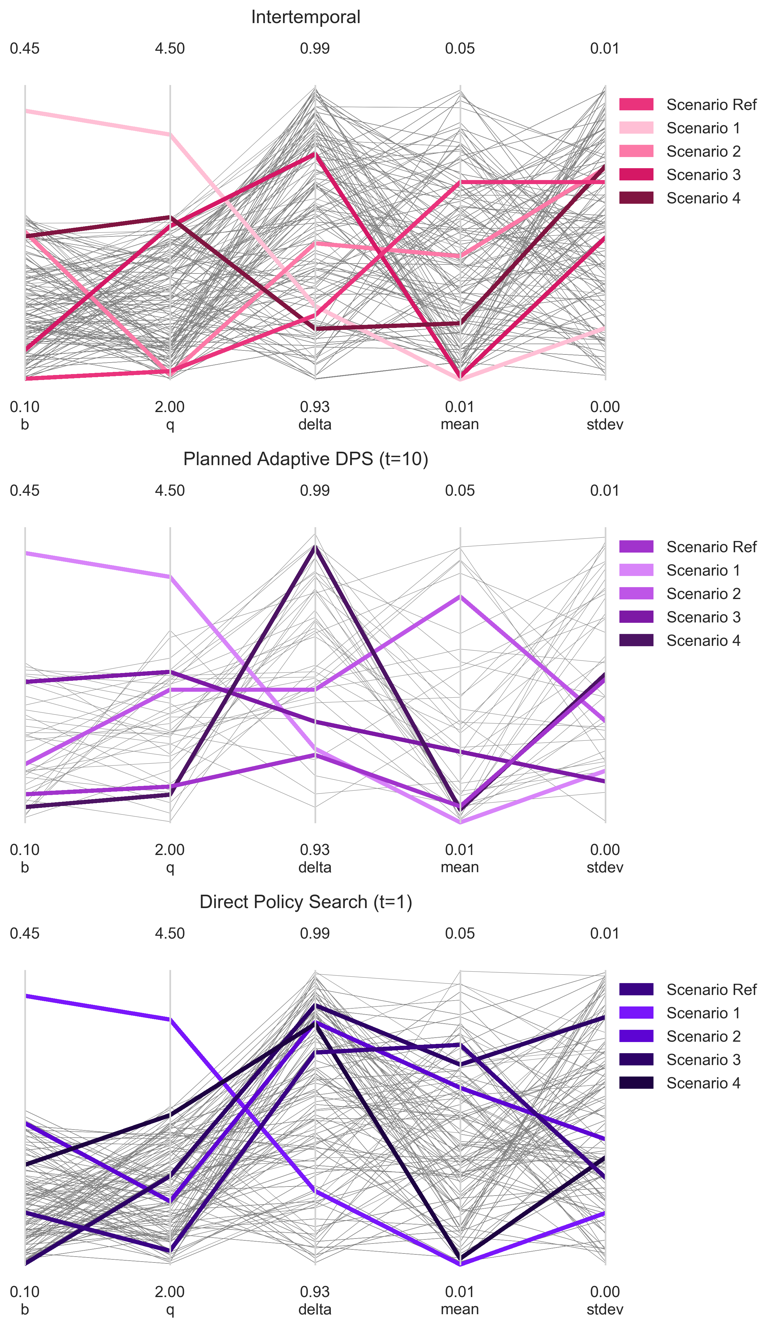
\includegraphics[width=0.75\linewidth]{scenarioselect/selected_scenarios}
        \caption[Uncertainty values used to select reference scenarios for multi-scenario MORDM]{Uncertainty values for the maximally diverse scenarios for each variation of the lake problem}
        \label{fig:selected-scenarios}
    \end{figure}
    
    \begin{table}[H]
        \centering
        \captionsetup{width=\textwidth}
        \caption[Reference Scenarios used for the intertemporal model variation]{Reference scenarios used for intertemporal analysis with the multi-Scenario MORDM method}
        \label{table:refscenario-inter}
        
        \setlength\arrayrulewidth{1pt}\arrayrulecolor{white}
        \rowcolors{2}{odd-row-blue}{even-row-blue}
        \begin{tabularx}{\textwidth}{|l|R|R|R|R|R|}
            \rowcolor{tudelft-dark-blue!80}
            {\color{white} Reference Scenario} & 
            \multicolumn{1}{|c|}{\color{white} b} & \multicolumn{1}{|c|}{\color{white} q} & \multicolumn{1}{|c|}{\color{white} mean} & \multicolumn{1}{|c|}{\color{white} stdev} & \multicolumn{1}{|c|}{\color{white} delta} \\ \hline
            
            1 & 0.2760 & 3.0490 & 0.0039 & 0.0039 & 0.9310 \\ \hline
            2 & 0.1350 & 2.0255 & 0.0407 & 0.0029 & 0.9613 \\ \hline
            3 & 0.2704 & 2.4783 & 0.0169 & 0.0039 & 0.9631 \\ \hline
            4 & 0.1009 & 3.6789 & 0.0187 & 0.0037 & 0.9317 \\ \hline
        \end{tabularx}
    \end{table}

    \begin{table}[H]
        \centering
        \captionsetup{width=\textwidth}
        \caption[Reference Scenarios used for the planned adaptive DPS model variation]{Reference scenarios used for planned adaptive DPS analysis with the multi-Scenario MORDM method}
        \label{table:refscenario-adapt}
        
        \setlength\arrayrulewidth{1pt}\arrayrulecolor{white}
        \rowcolors{2}{odd-row-blue}{even-row-blue}
        \begin{tabularx}{\textwidth}{|l|R|R|R|R|R|}
            \rowcolor{tudelft-dark-blue!80}
            {\color{white} Reference Scenario} & 
            \multicolumn{1}{|c|}{\color{white} b} & \multicolumn{1}{|c|}{\color{white} q} & \multicolumn{1}{|c|}{\color{white} mean} & \multicolumn{1}{|c|}{\color{white} stdev} & \multicolumn{1}{|c|}{\color{white} delta} \\ \hline
            
            1 & 0.1771 & 2.4274 & 0.0232 & 0.0048 & 0.9691 \\ \hline
            2 & 0.2084 & 3.3540 & 0.0399 & 0.0049 & 0.9872 \\ \hline
            3 & 0.3326 & 3.6983 & 0.0344 & 0.0040 & 0.9312 \\ \hline
            4 & 0.3939 & 4.0342 & 0.0257 & 0.0049 & 0.9522 \\ \hline
        \end{tabularx}
    \end{table}
    
    \begin{table}[H]
        \centering
        \captionsetup{width=\textwidth}
        \caption[Reference Scenarios used for the DPS model variation]{Reference scenarios used for DPS analysis with the multi-Scenario MORDM method}
        \label{table:refscenario-dps}
        
        \setlength\arrayrulewidth{1pt}\arrayrulecolor{white}
        \rowcolors{2}{odd-row-blue}{even-row-blue}
        \begin{tabularx}{\textwidth}{|l|R|R|R|R|R|}
            \rowcolor{tudelft-dark-blue!80}
            {\color{white} Reference Scenario} & 
            \multicolumn{1}{|c|}{\color{white} b} & \multicolumn{1}{|c|}{\color{white} q} & \multicolumn{1}{|c|}{\color{white} mean} & \multicolumn{1}{|c|}{\color{white} stdev} & \multicolumn{1}{|c|}{\color{white} delta} \\ \hline
            
            1 & 0.2683 & 3.5029 & 0.0430 & 0.0027 & 0.9429 \\ \hline
            2 & 0.1009 & 3.6998 & 0.0453 & 0.0044 & 0.9481 \\ \hline
            3 & 0.2187 & 2.0506 & 0.0428 & 0.0025 & 0.9504 \\ \hline
            4 & 0.1620 & 3.8685 & 0.0388 & 0.0022 & 0.9328 \\ \hline
        \end{tabularx}
    \end{table}

    \subsection{MORO}
    The MORO framework makes the most effort to incorporate considerations of robustness in the policy evaluation process, and does so in two steps. First, each alternative policy option is evaluated over a set of more than one scenarios; this study uses 50 scenarios for evaluation. Given the alternative's performance across those 50 scenario, policy alternatives are then used to calculate robustness values for each outcome of interest. These robustness values are then used to determine whether an alternative belongs to the set of non-dominated alternatives that the search process is building. The robustness definition in the search process is the same as is specified in \cref{step0-robust}, where a value between 0 and 1 is calculated that indicates the fraction of scenarios that meet the robustness threshold for each outcome of interest. By using robust values in the search process to determine the effectiveness of a potential policy alternative, it is more likely to build a set of alternatives that meet the robustness criteria that are targeted by decision makers. 

\section{Non-Dominated Selection of Alternatives} \label{step2-pareto}
Because there is an element of randomness to the MOEA's process, through the selection of the starting population of the search using a Latin Hypercube sampling across the decision lever space, this analysis will include multiple repetitions of each search in order to both study and manage the impact of the randomly selected starting population on the resulting set of non-dominated policy alternatives. Due to computational constraints, the number of variations changes depending on the method considered. Selected values are based on the computational requirements of that method and on the variation observed across searches. 

\begin{itemize}
    \item \textbf{MORDM}: 50 repetitions used
    \item \textbf{Multi-Scenario MORDM}: 20 repetitions per reference scenario used
    \item \textbf{MORO}: 10 repetitions used
\end{itemize}

Once the defined number of repetitions is complete, the resulting set of non-dominated policy alternatives is subjected to a final sort to build the ultimate set of non-dominated solutions. The algorithm used is also epsilon-based and uses the same configuration as the search algorithm \citep{Deb2002, Deb2005, Woodruff2013}. This final selection process results in a set of non-dominated policy alternatives that is not affected by the value of the random seed used. 